\documentclass[final,hyperref={pdfpagelabels=false}]{beamer}
\mode<presentation> { \usetheme{hhucn} }

\usepackage[scaled=.90]{helvet}  % Alternative font for HHU font 'Celeste'
\usepackage{grffile}  % to support file names with multiple dots in it.
\usepackage[english]{babel}
\usepackage[utf8]{inputenc}
\usepackage{amsmath,amsthm, amssymb, latexsym}
\usepackage{wrapfig}
\usepackage{subfigure}
\usepackage{array,booktabs,tabularx}
\usepackage[orientation=portrait,size=a1,scale=1.4,debug]{beamerposter}

% change list indention level
\setdefaultleftmargin{3em}{}{}{}{}{}
\providecommand\thispdfpagelabel[1]{}

%%%%%%%%%%%%%%%%%%%%%%%%%%%%%%%%%%%%%%%%%%%%%%%%%%%%%%%%%%%%%%%%%%%%%%%%%%%%%%%%%%%%%%
% Title, author, institute, and emails here.

\title{\huge \textcolor{hhublau}{
        Distributing Distributed Revision Control Systems
      }}
\author{\textcolor{hhublau}{
        Philipp Hagemeister, Martin Mauve
      }}
\institute[HhuAndWue]{\textcolor{hhublau}{
  \begin{tabular}[h]{c}
    Computer Networks Group
    Heinrich Heine University, D\"usseldorf, Germany \\
    \{hagemeister, mauve\}@cs.uni-duesseldorf.de
  \end{tabular}
}}

\date[Nov 7th, 2016]{Nov 7th, 2016}


%%%%%%%%%%%%%%%%%%%%%%%%%%%%%%%%%%%%%%%%%%%%%%%%%%%%%%%%%%%%%%%%%%%%%%%%%%%%%%%%%%%%%%
% Abstract
\newcommand{\printabstract}{Current revision control systems are commonly used in a distributed fashion but rely on centralized stores and low-latency communication. In this work we evaluate how they
would fare in fully distributed high latency networks such as delay tolerant networks (DTNs). We show that current revision control systems impose significant costs under these conditions even in moderately-sized networks. By simplifying/improving the merging process, these costs can be reduced. We also show that speeding up \textit{or slowing down} communication can reduce the costs significantly.
}


%%%%%%%%%%%%%%%%%%%%%%%%%%%%%%%%%%%%%%%%%%%%%%%%%%%%%%%%%%%%%%%%%%%%%%%%%%%%%%%%%%%%%%
% Conference
\newcommand{\printconference}{
  The 41st IEEE Conference on Local Computer Networks (LCN)\\
  \vspace{1ex}
  Dubai, United Arab Emirates, November 2016
}


%%%%%%%%%%%%%%%%%%%%%%%%%%%%%%%%%%%%%%%%%%%%%%%%%%%%%%%%%%%%%%%%%%%%%%%%%%%%%%%%%%%%%%
\newlength{\columnheight}
\setlength{\columnheight}{105cm}


%%%%%%%%%%%%%%%%%%%%%%%%%%%%%%%%%%%%%%%%%%%%%%%%%%%%%%%%%%%%%%%%%%%%%%%%%%%%%%%%%%%%%%
\begin{document}
\begin{frame}
\begin{columns}
\begin{column}{.9\textwidth}  % Width for main content of the poster.

  {\Large
  Defeat censorship by using decentralized revision control systems (e.g. \textit{git}) in delay tolerant networks
  }

  \vspace{10mm}
  \begin{columns}
  \begin{column}{.5\textwidth}
      {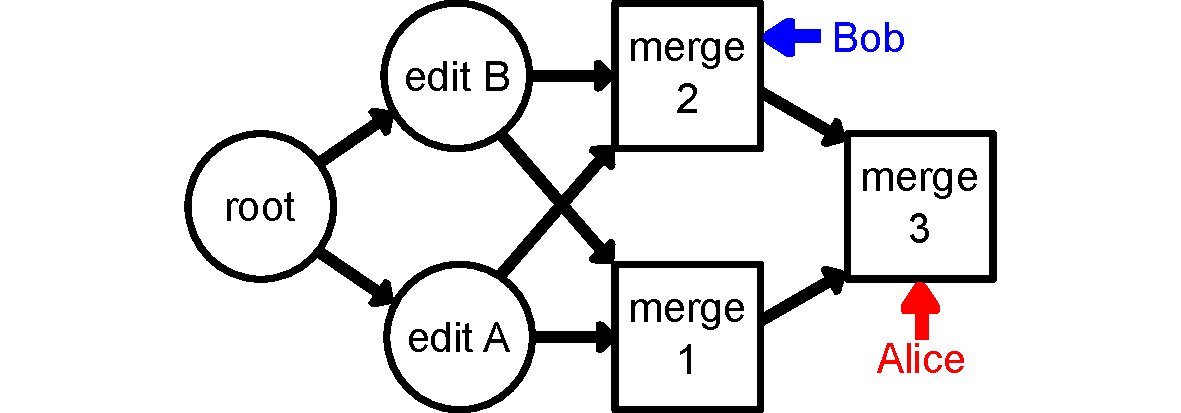
\includegraphics[width=0.7\linewidth]{fig/grcs}}
  \end{column}
  \begin{column}{.5\textwidth}
      {
\includegraphics[width=\linewidth]{fig/transfer_via}}
  \end{column}
  \end{columns}

  \vspace{10mm}
  \begin{beamercolorbox}[leftskip=0.5em,rightskip=0.5em,colsep*=.75ex,sep=0.5ex,vmode]{block body}%
  \vspace{0.2em}
    Real-world decentralized revision control systems have a small number of centralized hubs, which makes them vulnerable to censorship. When a revision control system is used in a distributed fashion, users must merge content to get a consistent view - but \textbf{how many merges} are required?
  \vspace{0.2em}
  \end{beamercolorbox}

  \vspace{10mm}
  \begin{columns}
  \begin{column}{.3\textwidth}
    \begin{center}
      When merging is not transitive:\\
      (hint: with git, it isn't)
    \end{center}

    \begin{figure}
      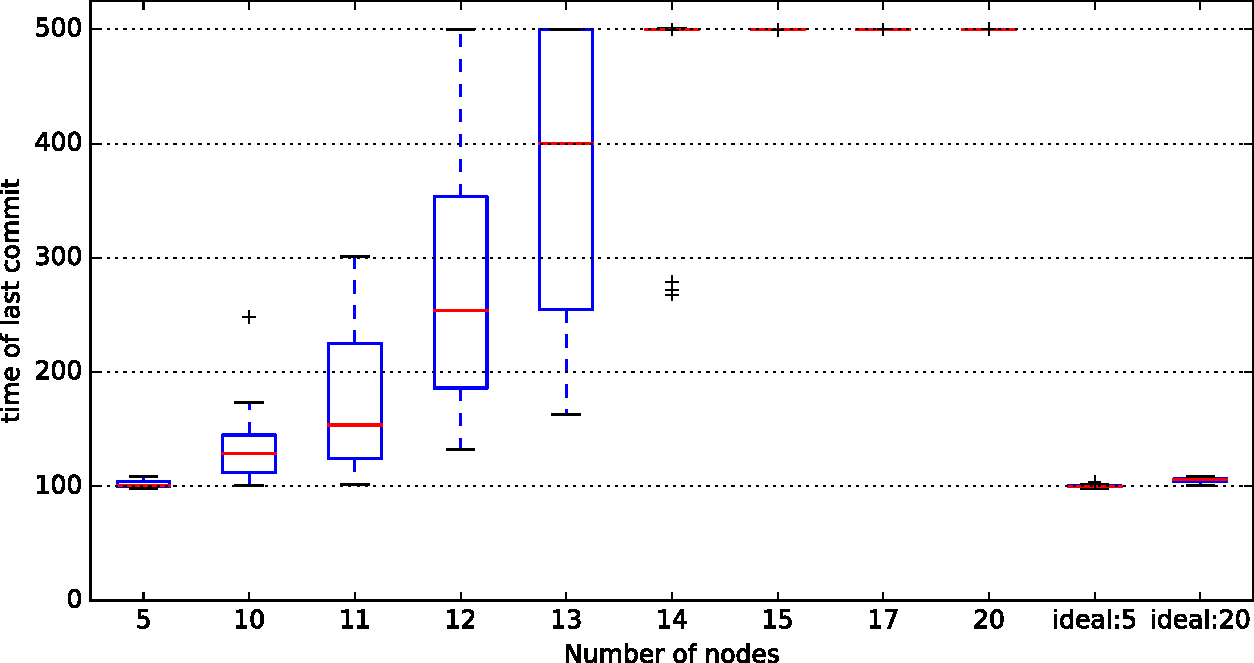
\includegraphics[width=\linewidth]{fig/dumb_sunset_n_scale_last.pdf}
    \end{figure}
  \end{column}
  \begin{column}{.3\textwidth}
    \begin{center}
    Clearly, users would not merge forever, \\
    but either ignore ...
    \end{center}
    \begin{figure}
      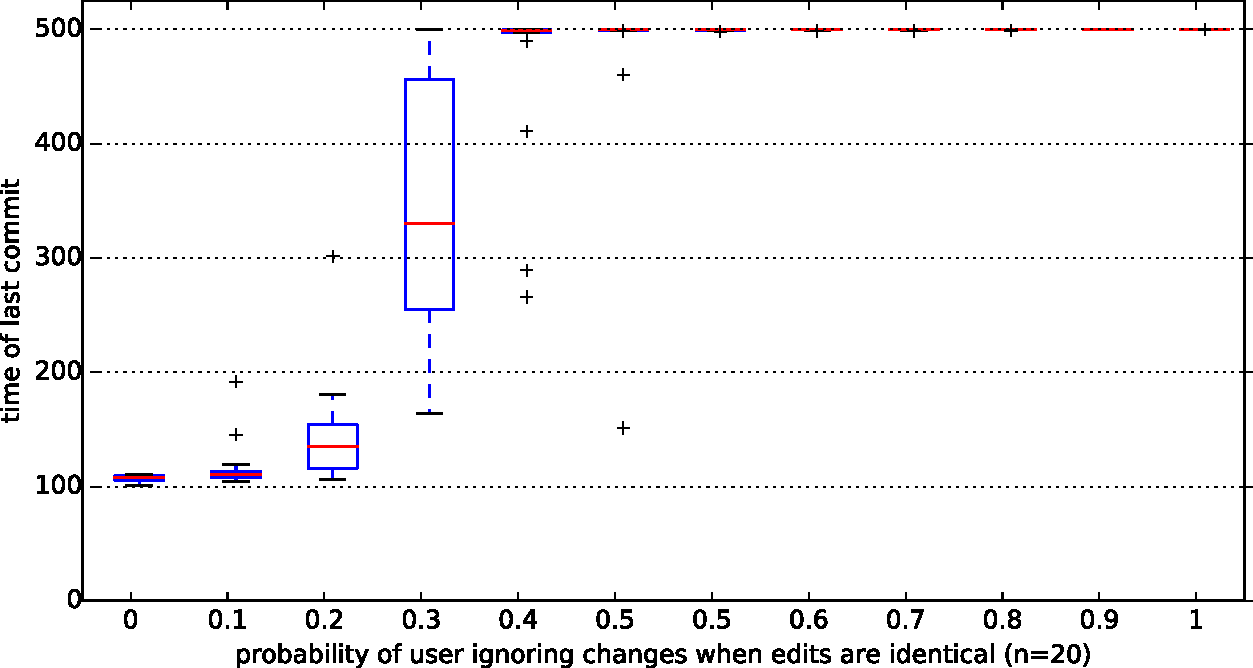
\includegraphics[width=\linewidth]{fig/bored_n=20.pdf}
    \end{figure}
  \end{column}
  \begin{column}{.3\textwidth}
    \begin{center}
    ... or simply accept remote changes \\
    without merging anymore
    \end{center}
    \begin{figure}
      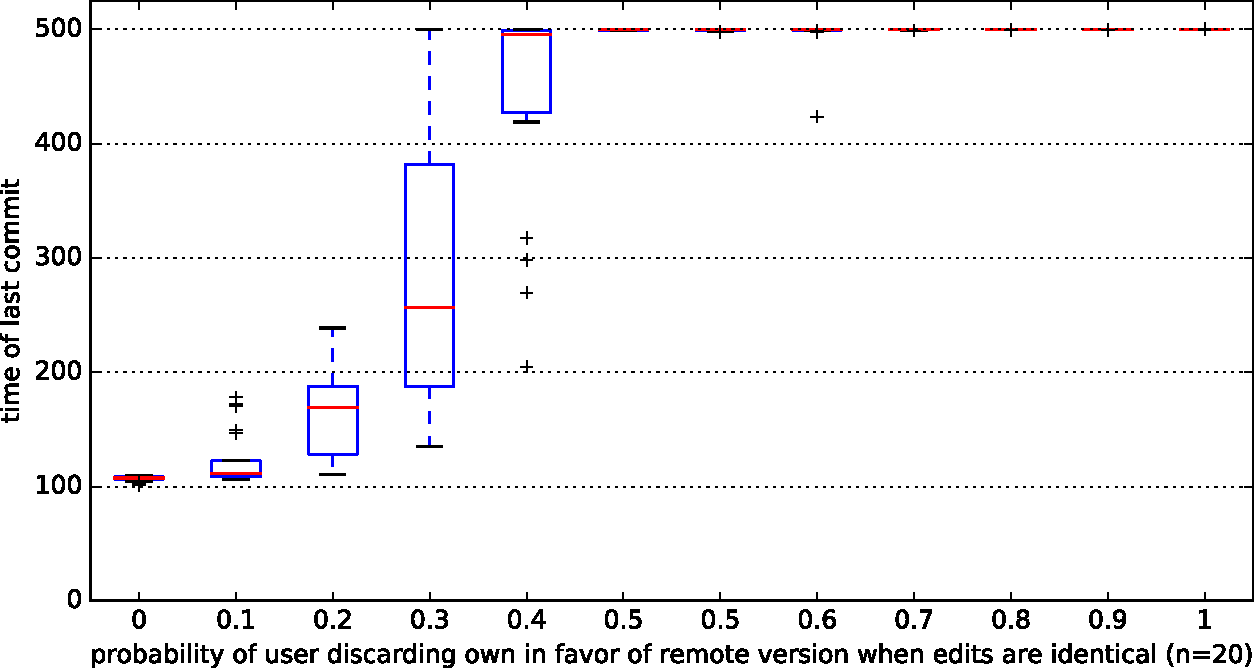
\includegraphics[width=\linewidth]{fig/bored_accept_n=20.pdf}
    \end{figure}
  \end{column}

  \end{columns}
  \vspace{10mm}
  \begin{center}
  Infinite merges even without new content, starting at {\raise.17ex\hbox{$\scriptstyle\sim$}}15 users!\hspace{2cm}So let's also look at an ideal (transitive\&commutative) merging function:
  \end{center}

  \vspace{8mm}
  \textbf{What factors impact the number of merges?}
  \vspace{5mm}

  \begin{columns}
  \begin{column}{.3\textwidth}
    \begin{center}
      Number of nodes (constant content):
    \end{center}
    \begin{figure}
      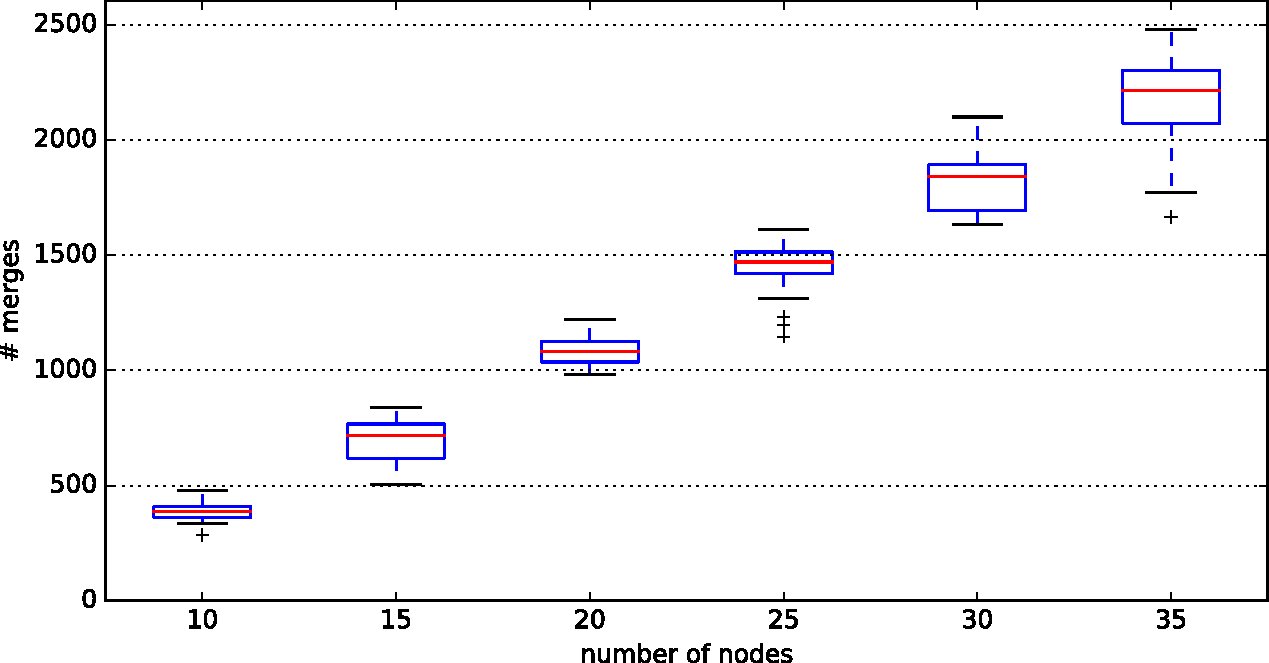
\includegraphics[width=\linewidth]{fig/n_with_same_edits.pdf}
    \end{figure}
  \end{column}
  \begin{column}{.3\textwidth}
    \begin{center}
    Meeting frequency (ideal, small network):
    \end{center}
    \begin{figure}
      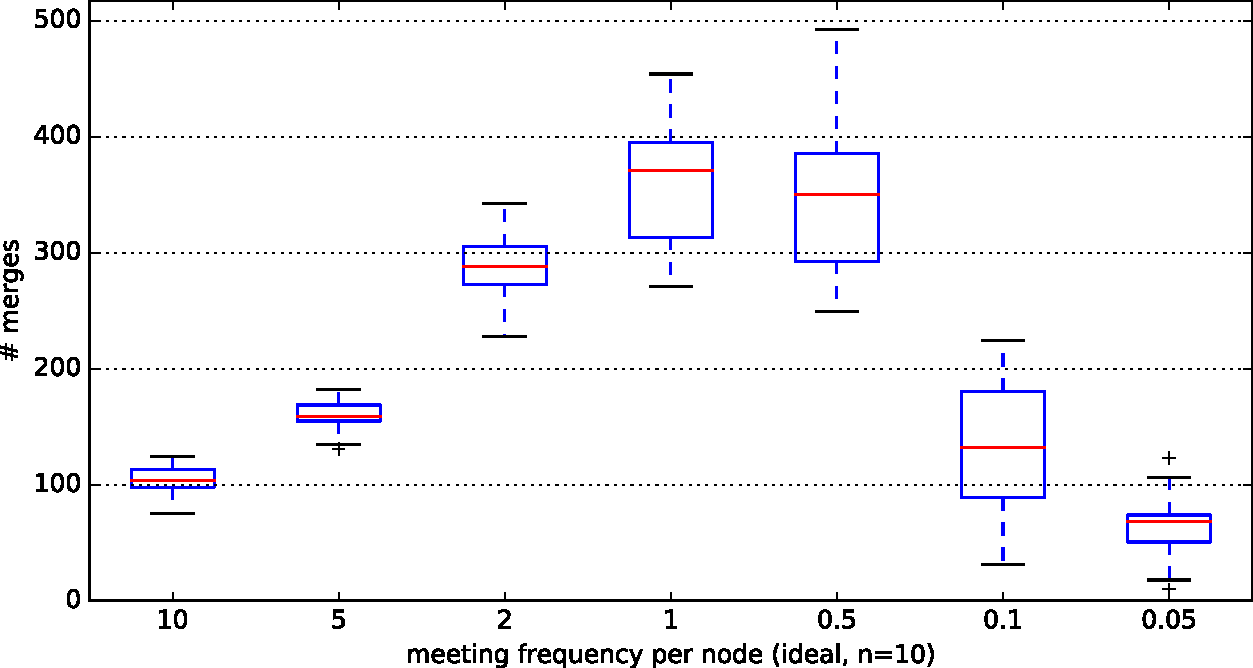
\includegraphics[width=\linewidth]{fig/global_meeting_frequency_n=10.pdf}
    \end{figure}
  \end{column}
  \begin{column}{.3\textwidth}
    \begin{center}
    Meeting frequency (default, small network):
    \end{center}
    \begin{figure}
      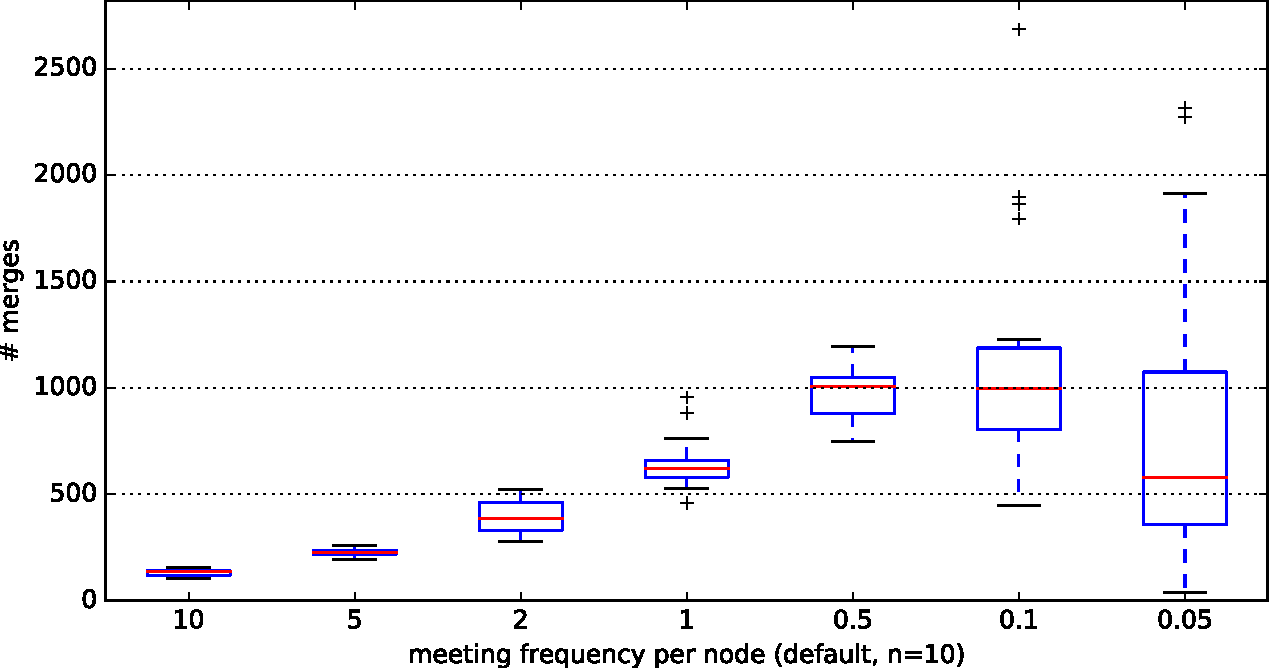
\includegraphics[width=\linewidth]{fig/dumb_meeting_frequency_n=10.pdf}
    \end{figure}
  \end{column}
  \end{columns}

  \begin{columns}
  \begin{column}{.3\textwidth}
    \begin{center}
       Nodes merge before going on:
    \end{center}
    \begin{figure}
      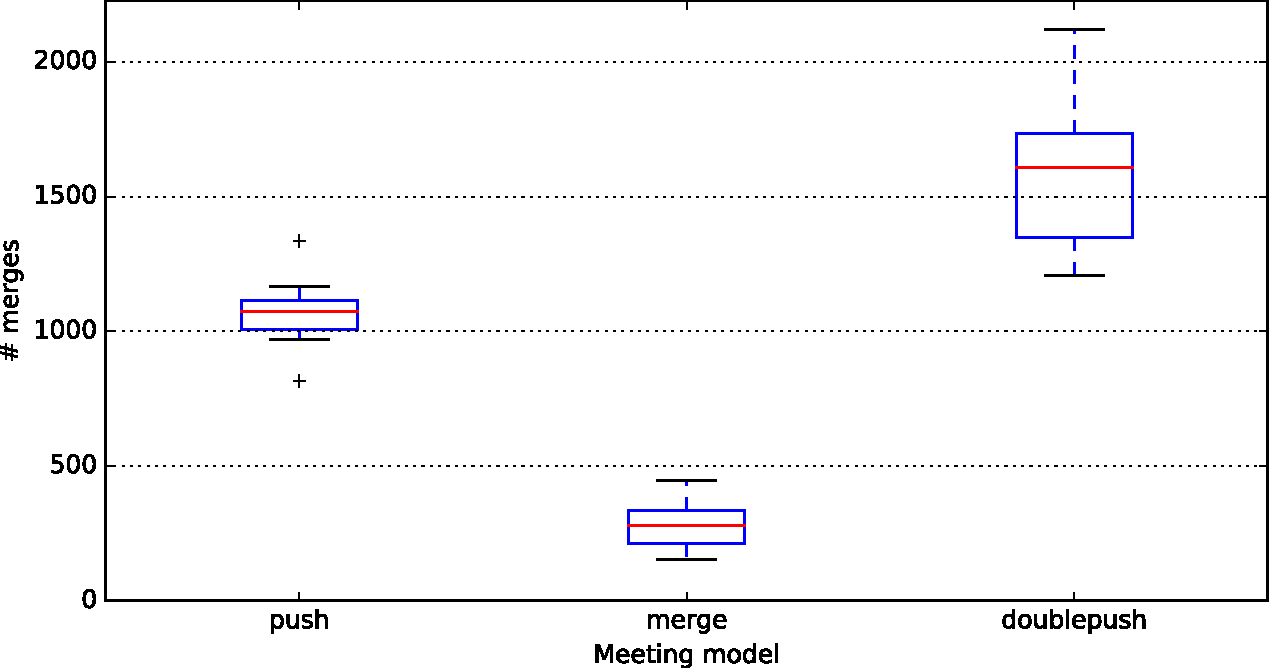
\includegraphics[width=\linewidth]{fig/bidi_n=20.pdf}
    \end{figure}
  \end{column}
  \begin{column}{.3\textwidth}
    \begin{center}
    Meeting frequency (ideal, large network):
    \end{center}
    \begin{figure}
      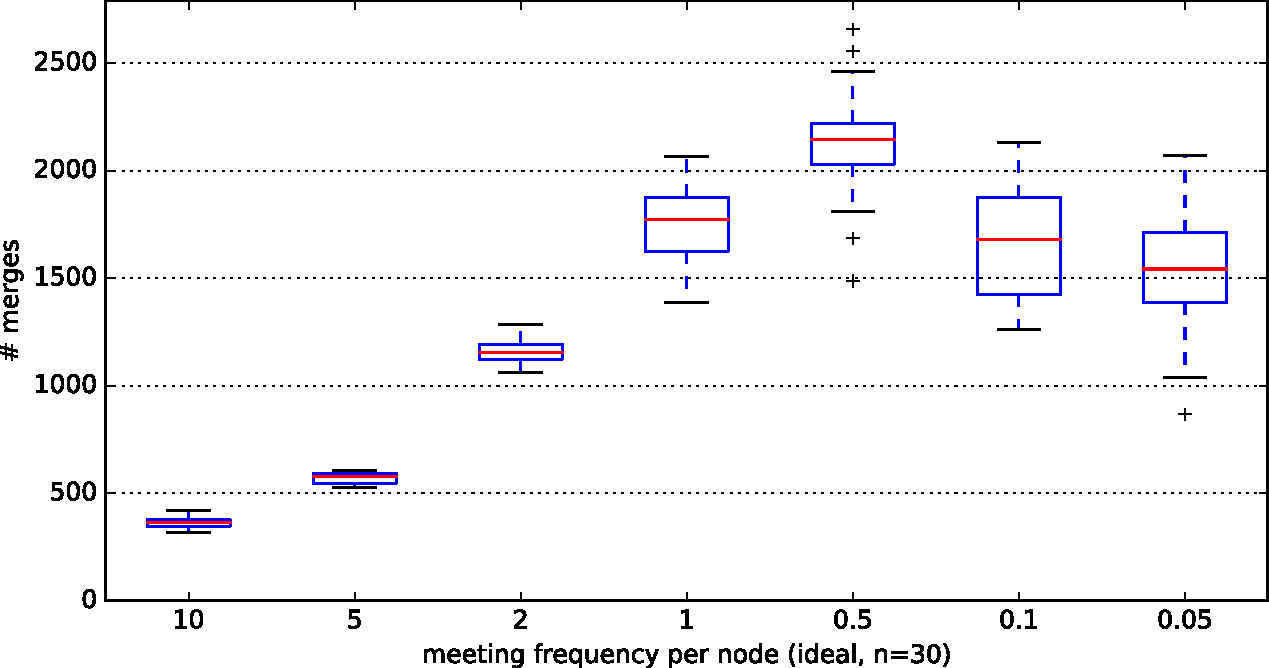
\includegraphics[width=\linewidth]{fig/global_meeting_frequency_n=30.pdf}
    \end{figure}
  \end{column}
  \begin{column}{.3\textwidth}
    \begin{center}
    Meeting frequency (default, large network):
    \end{center}
    \begin{figure}
      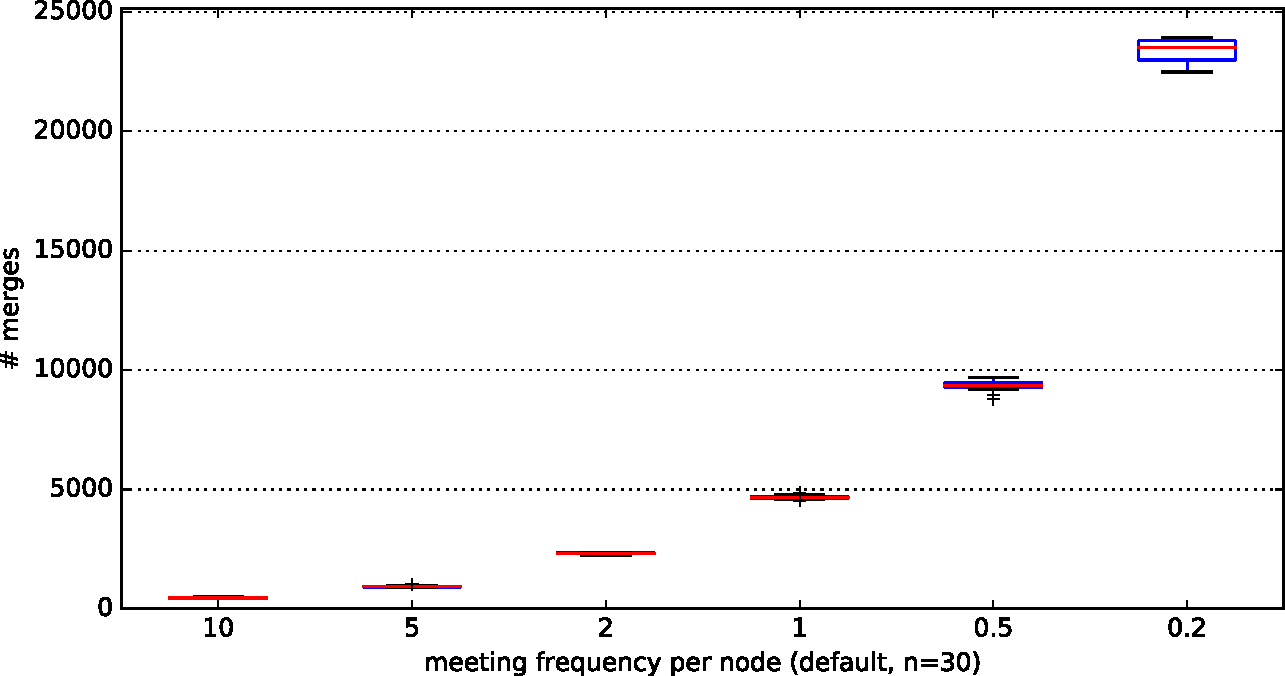
\includegraphics[width=\linewidth]{fig/dumb_meeting_frequency_n=30.pdf}
    \end{figure}
  \end{column}

  \end{columns}

  \vspace{10mm}
  \begin{center}
  
  \end{center}


  \vspace{1mm}
  \begin{beamercolorbox}[leftskip=0.5em,rightskip=0.5em,colsep*=.75ex,sep=0.5ex,vmode]{block body}%
  \vspace{0.2em}
  Surprisingly, with an ideal merging function (\textit{darcs} may be a real-world example) the number of merges increases only linearly. \\
  Bidirectional merging and meeting frequency have an impact on merge counts, easily 10x. \\
  \vspace{0.2em}
  \end{beamercolorbox}

  \vspace{1.5cm}
  \begin{center}
  \textbf{Future research needed on how to prevent merging in the first place, even in a fully distributed system with \textit{many} branches!}
  \end{center}

\end{column}
\end{columns}
\end{frame}
\end{document}


%%%%%%%%%%%%%%%%%%%%%%%%%%%%%%%%%%%%%%%%%%%%%%%%%%%%%%%%%%%%%%%%%%%%%%%%%%%%%%%%%%%%%%%%%%%%%%%%%%%%
